\documentclass[11pt,a4paper]{report}

\usepackage[utf8]{inputenc}
\usepackage[T1]{fontenc}
\usepackage[english]{babel}
\usepackage{geometry}
\geometry{top=2.3cm,bottom=2.3cm,left=2.5cm,right=2.5cm}
\usepackage{booktabs}
\usepackage{longtable}
\usepackage{tabularx}
\usepackage{array}
\usepackage{float}
\usepackage{caption}
\usepackage{enumitem}
\usepackage{xcolor}
\usepackage{tikz}
\usetikzlibrary{arrows.meta,positioning,shapes.geometric}
\usepackage{listings}
\usepackage{hyperref}
\usepackage{fancyhdr}
\usepackage{setspace}

\newcolumntype{P}[1]{>{\raggedright\arraybackslash}p{#1}}
\newcommand{\codeid}[1]{\path{#1}}

\definecolor{fptorange}{RGB}{242,113,37}
\definecolor{darkblue}{RGB}{0,51,102}
\definecolor{lightblue}{RGB}{228,239,250}
\definecolor{lightorange}{RGB}{255,239,224}
\definecolor{lightgreen}{RGB}{231,246,232}

\hypersetup{
  colorlinks=true,
  linkcolor=darkblue,
  urlcolor=blue,
  citecolor=darkblue,
  pdftitle={IoT-Based Multi-Sensor Anti-Theft System for Kitchen Area},
  pdfauthor={Group 6 - IOT102},
  pdfsubject={Current Version 3 scientific project report}
}

\pagestyle{fancy}
\fancyhf{}
\fancyhead[L]{IOT102 - Group 6}
\fancyhead[R]{Kitchen Security System - Version 3}
\fancyfoot[C]{\thepage}
\setlength{\headheight}{14pt}
\setstretch{1.08}
\emergencystretch=2em
\raggedbottom
\setlist[itemize]{leftmargin=1.5em,itemsep=0.25em}
\setlist[enumerate]{leftmargin=1.7em,itemsep=0.25em}
\renewcommand{\arraystretch}{1.2}

\lstset{
  basicstyle=\ttfamily\small,
  frame=single,
  breaklines=true,
  columns=fullflexible,
  backgroundcolor=\color{gray!5},
  keywordstyle=\color{darkblue}\bfseries,
  commentstyle=\color{green!40!black}
}

\tikzset{
  block/.style={draw,rounded corners,align=center,minimum width=3.2cm,
    minimum height=1.05cm,font=\small},
  arrow/.style={-{Latex[length=2.5mm]},thick}
}

\begin{document}
\pagenumbering{Alph}

% ------------------------------------------------------------------
% TITLE PAGE
% ------------------------------------------------------------------
\begin{titlepage}
\begin{center}
  \vspace*{0.5cm}
  {\Large\bfseries\textcolor{fptorange}{FPT UNIVERSITY}}\\[0.2cm]
  {\large Ho Chi Minh City Campus}\\[1.8cm]

  {\Huge\bfseries\textcolor{darkblue}{IoT-BASED MULTI-SENSOR}}\\[0.25cm]
  {\Huge\bfseries\textcolor{darkblue}{ANTI-THEFT SYSTEM}}\\[0.25cm]
  {\Huge\bfseries\textcolor{darkblue}{FOR KITCHEN AREA}}\\[1.5cm]

  {\Large\bfseries\textcolor{fptorange}{ACADEMIC PROJECT REPORT}}\\[0.3cm]
  {\large Course: IOT102 - Internet of Things}\\
  {\large Class: SE2034}\\
  {\large Technical baseline: Firmware Version 3}\\[1.6cm]

  \textbf{\large Prepared by Group 6}\\[0.4cm]
  \begin{tabular}{clll}
    \toprule
    \textbf{No.} & \textbf{Full Name} & \textbf{Student ID} & \textbf{Project Role}\\
    \midrule
    1 & Ngo Gia Long & SE190732 & Group Leader\\
    2 & Nguyen Nhat Anh & SE192077 & Hardware Engineer\\
    3 & Vo Tran Cong Danh & SE190824 & Software Developer\\
    4 & Nguyen An Vuong & SE190996 & Testing and Support\\
    \bottomrule
  \end{tabular}

  \vfill
  {\large FPT University, Ho Chi Minh City}\\
  {\large July 2026}
\end{center}
\end{titlepage}

% ------------------------------------------------------------------
% FRONT MATTER
% ------------------------------------------------------------------
\pagenumbering{roman}

\chapter*{Abstract}
\addcontentsline{toc}{chapter}{Abstract}
This report presents the current Version 3 implementation of an IoT-based
multi-sensor anti-theft system for a residential kitchen. The prototype is
built around a Freenove ESP32-S3 WROOM board with an OV3660 camera. A Passive
Infrared (PIR) sensor and an ultrasonic sensor are jointly used to detect
intrusion, while a Light Dependent Resistor (LDR) and the ultrasonic sensor
form a separate anti-sabotage condition. A DS1307 real-time clock supplies the
time used by the dashboard and automatic arm/disarm schedule. Local responses
are produced by an active buzzer and red/green status LEDs.

Remote functions are implemented through Arduino IoT Cloud, Telegram, Google
Apps Script, Gmail, and an optional Gemini image-analysis request. The camera
supports manual and event-driven still-image capture. Gemini is constrained by
the firmware prompt to classify an image as PERSON or NONE; it does not
identify a face, determine identity, or decide that a person is an intruder.
Google Apps Script records device heartbeat messages, sends one offline and
one recovery email for ordinary connection loss, and raises a critical event
only when heartbeat loss follows an active sabotage event. SOS and critical
events require Parent/Admin confirmation before a report is sent to a
configured demonstration contact.

The report was revised by static traceability analysis of the Version 3
firmware, the 33 Arduino Cloud properties, and the Apps Script backend. It
therefore distinguishes implemented code paths from runtime results that still
require hardware evidence. The analysis also identifies current limitations:
blocking network calls, third-party data processing, no persistent alarm state
across reboot, no face recognition, no video recording, and a timing conflict
between AI follow-up scheduling and the camera cooldown.

\noindent\textbf{Keywords:} Internet of Things; home security; multi-sensor
fusion; ESP32-S3; OV3660; intrusion detection; anti-sabotage; human
confirmation; device heartbeat.

\clearpage
\tableofcontents
\listoffigures
\listoftables
\clearpage
\pagenumbering{arabic}

% ------------------------------------------------------------------
\chapter{Introduction}
% ------------------------------------------------------------------

\section{Background}
Residential security systems must operate under uncertainty. Motion can be
generated by residents, animals, curtains, or environmental effects; network
services can fail independently from local sensors; and a camera image may be
ambiguous. A kitchen is a useful prototype environment because it may include
external windows or doors and because occupants often want remote awareness
when nobody is at home.

The project is defined as a configurable IoT security prototype rather than an
autonomous law-enforcement system. The user enables protection manually or
through an RTC schedule. When a physical condition is sustained for the
required time, the device latches an alert, activates local outputs, records
context, and may send remote evidence. Human confirmation remains necessary
before the demonstration escalation path is completed.

\section{Problem Statement}
The current work addresses four engineering problems:
\begin{enumerate}
  \item A single sensor can produce ambiguous evidence; two physical signals
        should be required for intrusion and sabotage triggers.
  \item A local alarm alone is insufficient when the user is away; status and
        evidence must be available remotely.
  \item A compromised or disconnected device may stop reporting; the backend
        must use the time of the last heartbeat to detect this condition.
  \item Camera images, location data, and event logs are sensitive; the design
        must explicitly identify where third-party services process them.
\end{enumerate}

\section{Objectives}
The Version 3 objectives are:
\begin{itemize}
  \item detect an armed intrusion using PIR and ultrasonic confirmation;
  \item detect a possible sensor-covering attempt using LDR and distance;
  \item maintain local audible and visual alert outputs without Internet;
  \item support manual and automatic still-image capture;
  \item use AI only as supplementary PERSON/NONE image classification;
  \item provide Telegram, email, and Arduino Cloud status channels;
  \item monitor periodic device heartbeat and distinguish ordinary offline
        status from post-sabotage critical status;
  \item support Child and Parent/Admin SOS sources and human-confirmed
        demonstration escalation;
  \item allow Parent/Admin to configure the system remotely.
\end{itemize}

\section{Scope and Non-Scope}
\textbf{In scope} are the Freenove ESP32-S3 WROOM, OV3660 still camera, PIR,
HY-SRF05/HC-SR04-compatible ultrasonic sensor, analog LDR, DS1307, LEDs,
active buzzer, Arduino IoT Cloud, Telegram, Gemini, and Google Apps Script.

\textbf{Outside Version 3 scope} are RFID, trusted-phone BLE, Wi-Fi/MAC
scanning, fire or gas detection, face recognition, video recording, automatic
contact with a real public authority, a private mobile application, and
multi-room synchronization. These items must not be presented as completed
features.

\section{Main Contributions}
The current prototype contributes:
\begin{enumerate}
  \item separate, sustained multi-sensor rules for intrusion and sabotage;
  \item local-first alert behavior that is not cleared by a failed API call;
  \item event-driven camera capture and optional image classification;
  \item a server-side heartbeat correlation rule for sabotage followed by
        connection loss;
  \item an escalation workflow that preserves human confirmation and does not
        automatically silence the local alarm.
\end{enumerate}

% ------------------------------------------------------------------
\chapter{Research and Verification Method}
% ------------------------------------------------------------------

\section{Evidence Sources}
This revision uses the following source hierarchy:
\begin{enumerate}
  \item the Version 3 Arduino sketch;
  \item the generated \texttt{thingProperties.h} Cloud contract;
  \item the Version 3 Google Apps Script backend;
  \item the current software requirements specification;
  \item the June 2026 PDF only as historical context.
\end{enumerate}

\section{Static Traceability Method}
Each scientific claim about the current system was mapped to a constant,
property, function, or backend state transition. Pin numbers were read from
preprocessor definitions. Detection conditions were traced from
\texttt{updateIntrusionLogic()} and \texttt{updateSabotageLogic()}. Camera,
Telegram, Gemini, and Apps Script behaviors were traced through their request
functions and status branches. Backend states were traced from event handlers,
Script Properties, and the time-based heartbeat monitor.

\section{Evidence Boundary}
The revision confirms that code paths exist; it does not by itself prove
sensor accuracy, AI accuracy, network latency, or long-term stability. Runtime
claims require board logs, dashboard screenshots, Telegram photos, email
records, and repeatable test conditions. Consequently, Chapter 7 reports
static verification results and a runtime validation plan rather than
fabricated PASS results.

% ------------------------------------------------------------------
\chapter{System Architecture and Hardware}
% ------------------------------------------------------------------

\section{Current Architecture}
\begin{figure}[H]
\centering
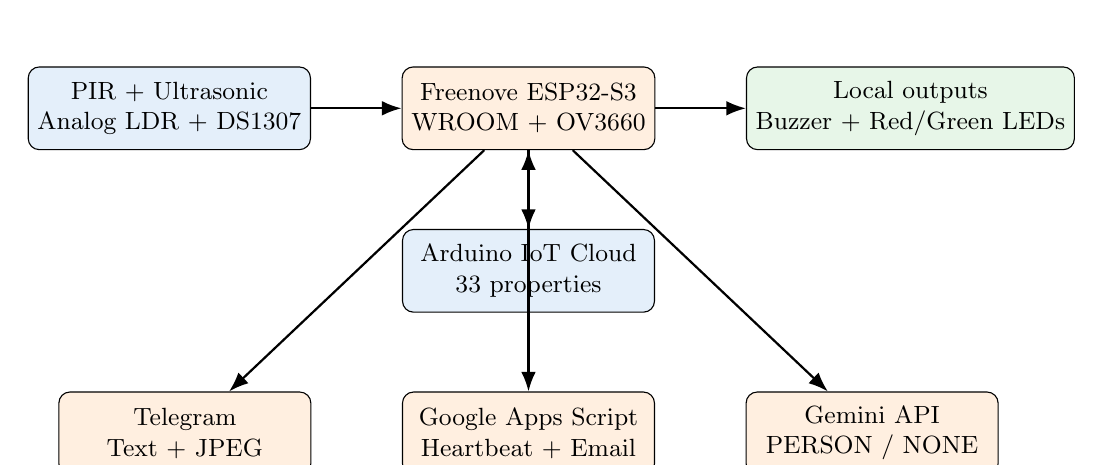
\begin{tikzpicture}[node distance=1.0cm and 1.15cm]
  \node[block,fill=lightblue] (sensors) {PIR + Ultrasonic\\Analog LDR + DS1307};
  \node[block,fill=lightorange,right=of sensors] (esp) {Freenove ESP32-S3\\WROOM + OV3660};
  \node[block,fill=lightgreen,right=of esp] (local) {Local outputs\\Buzzer + Red/Green LEDs};
  \node[block,fill=lightblue,below=of esp] (cloud) {Arduino IoT Cloud\\33 properties};
  \node[block,fill=lightorange,below left=of cloud] (tg) {Telegram\\Text + JPEG};
  \node[block,fill=lightorange,below=of cloud] (gas) {Google Apps Script\\Heartbeat + Email};
  \node[block,fill=lightorange,below right=of cloud] (ai) {Gemini API\\PERSON / NONE};

  \draw[arrow] (sensors) -- (esp);
  \draw[arrow] (esp) -- (local);
  \draw[arrow] (esp) -- (cloud);
  \draw[arrow] (cloud) -- (esp);
  \draw[arrow] (esp) -- (tg);
  \draw[arrow] (esp) -- (gas);
  \draw[arrow] (esp) -- (ai);
\end{tikzpicture}
\caption{Version 3 system architecture and information paths}
\label{fig:architecture}
\end{figure}

\section{Hardware Components}
\begin{table}[H]
\centering
\caption{Current hardware baseline}
\begin{tabularx}{\textwidth}{p{3.2cm}p{3.8cm}X}
\toprule
\textbf{Component} & \textbf{Current Model/Mode} & \textbf{Purpose}\\
\midrule
Main controller & Freenove ESP32-S3 WROOM & Sensor processing, Wi-Fi,
Cloud synchronization, HTTPS clients, and local outputs\\
Camera & OV3660, JPEG & Still-image evidence; VGA with PSRAM and QVGA
without PSRAM\\
Motion sensor & PIR & Digital movement evidence\\
Distance sensor & HY-SRF05 or compatible HC-SR04 & Object distance and
very-close tamper evidence\\
Light sensor & Analog LDR module & Raw light value, light delta, and
covered-sensor condition\\
Real-time clock & DS1307 via I2C & Dashboard time and automatic schedule\\
Audible output & Active buzzer mode & Local warning using HIGH/LOW output\\
Visual outputs & Red and green LEDs & Alert and normal-state indication\\
\bottomrule
\end{tabularx}
\end{table}

\section{Pin Assignment}
\begin{longtable}{p{3.5cm}p{3.0cm}p{7.0cm}}
\caption{Version 3 pin assignment}\\
\toprule
\textbf{Function} & \textbf{GPIO} & \textbf{Implementation note}\\
\midrule
\endfirsthead
\toprule
\textbf{Function} & \textbf{GPIO} & \textbf{Implementation note}\\
\midrule
\endhead
LDR analog output & 1 & Read with 12-bit ADC resolution\\
PIR output & 40 & Digital input\\
RTC SDA / SCL & 41 / 42 & I2C bus for \texttt{RTC\_DS1307}\\
Ultrasonic TRIG / ECHO & 38 / 39 & Trigger output and echo input\\
Red / green LED & 14 / 21 & Alert and normal indicators\\
Active buzzer & 47 & \texttt{BUZZER\_USE\_TONE=false}\\
Camera XCLK & 15 & 10 MHz camera clock\\
Camera SIOD / SIOC & 4 / 5 & Camera control bus\\
Camera Y2--Y9 & 11, 9, 8, 10, 12, 18, 17, 16 & Eight-bit image data bus\\
Camera VSYNC / HREF / PCLK & 6 / 7 / 13 & Camera timing signals\\
\bottomrule
\end{longtable}

\section{Timing and Threshold Parameters}
\begin{table}[H]
\centering
\caption{Firmware timing and sensor constants}
\begin{tabularx}{\textwidth}{p{5.2cm}p{3.0cm}X}
\toprule
\textbf{Parameter} & \textbf{Value} & \textbf{Meaning}\\
\midrule
Sensor update interval & 500 ms & Target period for hardware snapshots\\
Boot grace interval & 3 s & Intrusion readings ignored after boot\\
Near-object threshold & 50 cm & Upper distance boundary for intrusion\\
Too-close threshold & 15 cm & Reserved for sabotage condition\\
Intrusion hold & 2 s & Condition must remain continuously true\\
Sabotage hold & 3 s & Condition must remain continuously true\\
LDR covered threshold & $\geq 2000$ by default & Configurable polarity in code\\
LDR abnormal delta & 500 ADC counts & Score and status signal only\\
Heartbeat interval & 10 s & Device-to-Apps-Script period\\
Heartbeat timeout & 40 s & Backend offline threshold\\
Red LED blink & 250 ms & Alert-state visual cadence\\
Camera cooldown & 1.5 s & Minimum time between capture attempts\\
AI follow-up interval & 1 s & Current scheduling interval\\
\bottomrule
\end{tabularx}
\end{table}

\section{RTC Interpretation}
The DS1307 continues timekeeping from its backup supply when the module is
correctly wired and powered as specified by the device datasheet
\cite{ds1307}. In this project the RTC is read through Adafruit RTClib
\cite{rtclib}. Firmware sets the clock to compile time only when the following
configuration flag is true, or when \texttt{rtc.isrunning()} is false:
\begin{center}
\codeid{FORCE_SET_RTC_TIME_ONCE}
\end{center}

The RTC does \emph{not} persist \texttt{alarm\_enabled}, alert latches, or the
previous system state. After reboot, runtime latches are cleared and Cloud
READWRITE values may later overwrite firmware defaults. Therefore, Version 3
must not be described as restoring the exact pre-failure security state.

% ------------------------------------------------------------------
\chapter{Cloud and Software Architecture}
% ------------------------------------------------------------------

\section{Arduino IoT Cloud Contract}
Arduino IoT Cloud provides remote property synchronization and dashboard
widgets \cite{arduino-cloud,arduino-iot-lib}. The generated contract contains
33 properties. Raw sensor values, intrusion score, threat level, and internal
event counters remain local in Version 3 and are not Cloud properties.

\small
\begin{longtable}{P{5.5cm}P{2.2cm}P{5.8cm}}
\caption{Arduino Cloud properties grouped by purpose}\\
\toprule
\textbf{Properties} & \textbf{Access} & \textbf{Purpose}\\
\midrule
\endfirsthead
\toprule
\textbf{Properties} & \textbf{Access} & \textbf{Purpose}\\
\midrule
\endhead
\codeid{alarm_status}, \codeid{system_armed} & Read & Overall protection state\\
\codeid{current_time}, \codeid{last_event} & Read & RTC time and latest event text\\
\codeid{intrusion_alert}, \codeid{sabotage_alert},
\codeid{critical_security_compromise} & Read & Latched security states\\
\codeid{device_health_status}, \codeid{heartbeat_status},
\codeid{last_heartbeat_time} & Read & Device and backend communication state\\
\codeid{notification_sent_status}, \codeid{photo_status} & Read & Delivery and camera feedback\\
\codeid{emergency_escalation_status},
\codeid{emergency_authority_message_status},
\codeid{home_address_configured} & Read & Backend confirmation/escalation state\\
\codeid{alarm_enabled} & Read/Write & Enables intrusion detection only\\
\codeid{schedule_enabled}, \codeid{auto_arm_hour},
\codeid{auto_arm_minute}, \codeid{auto_disarm_hour},
\codeid{auto_disarm_minute} & Read/Write & RTC schedule\\
\codeid{sensitivity_level} & Read/Write & Score/UX setting; not an intrusion gate\\
\codeid{camera_enabled}, \codeid{gemini_enabled},
\codeid{auto_photo_on_alert} & Read/Write & Camera and AI controls\\
\codeid{telegram_enabled}, \codeid{google_script_enabled},
\codeid{heartbeat_enabled} & Read/Write & Network-service controls\\
\codeid{manual_capture_photo}, \codeid{reset_alarm},
\codeid{sos_child}, \codeid{sos_adult} & Read/Write & Edge-triggered commands reset by firmware\\
\codeid{sos_authority_note} & Read/Write & Optional confirmation context\\
\bottomrule
\end{longtable}
\normalsize

\section{User Roles}
The project uses a Child-oriented dashboard and a Parent/Admin control
dashboard. The Child view exposes a simple SOS action and status, while the
Parent/Admin view exposes arming, scheduling, services, camera, reset, and
diagnostic status.

This division is a user-interface design. The firmware does not cryptographically
authenticate which role changed a property. Actual authorization depends on
Arduino Cloud account and dashboard-sharing permissions.

\section{Remote Services}
\begin{itemize}
  \item \textbf{Telegram Bot API:} sends text and JPEG images. The firmware
  uploads a new photo using multipart form data, consistent with the
  \texttt{sendPhoto} interface \cite{telegram-bot-api}.
  \item \textbf{Gemini API:} receives Base64 inline JPEG data and a constrained
  prompt. Official documentation identifies inline image data as a supported
  input method \cite{gemini-images}.
  \item \textbf{Google Apps Script:} accepts event parameters, stores compact
  event records in Script Properties, sends email, and exposes confirmation,
  status, resolve, and heartbeat-monitor endpoints. Script Properties are
  key-value storage scoped to the script \cite{apps-script-properties}.
\end{itemize}

\section{Backend Event States}
The backend state machine uses the following values:
\begin{center}
\codeid{IDLE}, \codeid{MONITORING}, \codeid{WAITING_CONFIRMATION},
\codeid{CONFIRMED}, \codeid{SENT}, \codeid{FAILED},
\codeid{NOT_CONFIGURED}, and \codeid{RESOLVED}.
\end{center}
Event records are retained for 24 hours and include an event identifier, type,
source, device, location, RTC time, server time, message, optional note, and
escalation timestamps.

% ------------------------------------------------------------------
\chapter{System Operation and Code-Level Logic}
% ------------------------------------------------------------------

\section{Boot and Main Loop}
At boot, firmware configures GPIO, clears runtime alert latches, starts the
DS1307, initializes the OV3660, creates Cloud properties, and begins Arduino
Cloud synchronization. The firmware initially enables the intrusion alarm,
Telegram, Apps Script, and heartbeat. It initially disables the camera,
Gemini, and automatic photo capture. Stored Cloud values may overwrite these
READWRITE defaults after connection.

The main loop calls \texttt{ArduinoCloud.update()}, handles serial input,
maintains Wi-Fi, processes heartbeat control and normal heartbeat, and every
500 ms reads sensors and evaluates the schedule and security logic. HTTPS
requests are synchronous; therefore, the nominal 500 ms interval is not a
hard real-time deadline during network calls.

\section{Intrusion Detection}
Intrusion is not activated by the score threshold. It requires the following
physical condition continuously for two seconds after the boot grace period:

\begin{lstlisting}
system_armed
AND pir_detected
AND distance_cm <= 50
AND distance_cm > 15
\end{lstlisting}

When triggered, \texttt{intrusion\_alert} is latched, the event is recorded,
the local alarm is activated, and an automatic camera request is queued.
Objects at 15 cm or less are reserved for the sabotage path.

The firmware still computes a diagnostic score: PIR $+2$, near object $+2$,
abnormal light delta $+1$, and night mode $+1$. The sensitivity value maps to
thresholds 5, 4, and 3, but neither the score nor the threshold gates
intrusion in Version 3.

\section{Pet Heuristic}
\texttt{pet\_detected} is true when an object is near while PIR and abnormal
light are false. It does not measure animal height, does not use AI, does not
reduce the intrusion score, and is not published to the Cloud. It is therefore
a demonstration heuristic, not validated pet classification.

\section{Anti-Sabotage Detection}
Sabotage is evaluated even when intrusion protection is disabled. The current
condition is:

\begin{lstlisting}
ldr_covered
AND distance_cm <= 15
AND condition_duration >= 3000 ms
\end{lstlisting}

The default LDR polarity treats ADC values at or above 2000 as covered. When
triggered, \texttt{sabotage\_alert} and \texttt{device\_tampered} are latched,
local outputs activate, a photo request is queued, and a
\texttt{sabotage\_alert} event is sent to Apps Script. The backend then
correlates any later heartbeat timeout with this active sabotage record.

\section{SOS and Human Confirmation}
\texttt{sos\_child} and \texttt{sos\_adult} are command properties. The
firmware maps them to sources \texttt{CHILD} and \texttt{PARENT\_ADULT}.
Either source latches SOS, activates local outputs, sends Telegram text, and
creates an Apps Script event. Version 3 does not calculate SOS levels 1--3.

Parent/Admin receives a confirmation link. Confirmation can add a note and may
send a report to a configured demonstration contact. Confirmation does not
reset the board. Only \texttt{reset\_alarm} clears local latches and turns off
the local alarm.

\section{Camera and Telegram}
The camera is initialized during setup even when \texttt{camera\_enabled} is
false. Capturing is allowed only when the camera switch is on, initialization
succeeded, and at least 1.5 seconds have elapsed since the previous attempt.
A stale framebuffer is discarded before obtaining a fresh image.

Manual capture is queued from a Cloud callback and processed in the main loop.
Automatic capture runs only when \texttt{auto\_photo\_on\_alert} is true.
Telegram applies independent 15-second cooldowns to intrusion, sabotage, SOS,
and manual categories.

\section{AI Image Classification}
When camera and Gemini controls are enabled and an API key exists, firmware
sends the JPEG inline as Base64. The prompt requests exactly \texttt{PERSON}
or \texttt{NONE}. The parsed firmware states are
\texttt{PERSON\_DETECTED} and \texttt{NO\_PERSON}; ambiguous or network
responses become error states.

The AI result is supplementary:
\begin{itemize}
  \item it does not change the sensor alert latch;
  \item it does not identify a face or determine identity;
  \item it does not label a detected person as an intruder;
  \item failure does not stop local buzzer/LED behavior;
  \item only automatic intrusion/sabotage captures may generate one
        AI-person email per current alert.
\end{itemize}

After PERSON is detected, firmware schedules three follow-up attempts at
one-second intervals without calling Gemini again. However, the camera rejects
captures within 1.5 seconds and the follow-up counter decreases even when an
attempt is rejected. Thus, Version 3 does not guarantee three successful
follow-up images. This is a code-level limitation.

\section{Heartbeat and Critical Correlation}
When Google Script and heartbeat controls are enabled, the board sends a
heartbeat every 10 seconds. Apps Script considers the device offline when the
last server-received heartbeat is older than 40 seconds. A time-based trigger
runs once per minute, so the email arrival time can exceed the nominal timeout.

Ordinary loss produces one family offline email. A new heartbeat produces one
recovery email. If an active sabotage record exists, timeout follows the
critical path instead: the backend creates or updates a critical event and
sends a confirmation email. It does not directly contact the demonstration
authority before confirmation.

Heartbeat demonstrates that the backend recently received a request. It does
not prove that every sensor and the camera are functioning.

\section{Alarm Priority and Reset}
Dashboard status priority is SOS, critical compromise, sabotage, intrusion,
armed, and disarmed. Alerts are latched and remain active until reset.
\texttt{alarm\_enabled} only gates intrusion; it does not disable SOS,
sabotage, critical state, or reset.

% ------------------------------------------------------------------
\chapter{Implementation Traceability}
% ------------------------------------------------------------------

\section{Firmware Function Mapping}
\small
\begin{longtable}{P{4.4cm}P{9.6cm}}
\caption{Requirement-to-code traceability}\\
\toprule
\textbf{Capability} & \textbf{Primary implementation functions}\\
\midrule
\endfirsthead
\toprule
\textbf{Capability} & \textbf{Primary implementation functions}\\
\midrule
\endhead
Sensor snapshot & \codeid{readHardwareSnapshot()},
\codeid{readUltrasonicDistanceCm()}, \codeid{calculateLdrCovered()}\\
RTC and schedule & \codeid{getRtcTimeString()},
\codeid{updateScheduleLogic()}\\
Intrusion & \codeid{updateIntrusionLogic()},
\codeid{triggerIntrusionAlert()}\\
Sabotage & \codeid{updateSabotageLogic()},
\codeid{triggerSabotageAlert()}\\
Local outputs & \codeid{applyAlarmOutputs()},
\codeid{setBuzzerPhysical()}, LED helpers\\
Camera & \codeid{initCamera()}, \codeid{captureFreshCameraFrame()},
\codeid{captureSecurityPhoto()}, \codeid{processCameraRequests()}\\
Gemini & \codeid{analyzePersonWithGemini()},
\codeid{writeBase64ToClient()}\\
Telegram & \codeid{sendTelegramMessage()},
\codeid{sendTelegramPhoto()}, \codeid{isTelegramAllowed()}\\
Heartbeat & \codeid{processGoogleAppsScriptHeartbeat()},
\codeid{processGoogleScriptHeartbeatMonitorControl()}\\
SOS/reset & \codeid{triggerSosAlert()}, \codeid{resetAllAlerts()}\\
Backend critical path & \codeid{monitorHeartbeatAfterSabotage()},
\codeid{handleCriticalRequest()}\\
Confirmation & \codeid{handleConfirmPage()},
\codeid{handleConfirmSend()}, \codeid{sendAuthorityEscalationEmail()}\\
\bottomrule
\end{longtable}
\normalsize

\section{Failure Handling}
\begin{table}[H]
\centering
\caption{Degraded-operation behavior}
\begin{tabularx}{\textwidth}{p{3.2cm}X}
\toprule
\textbf{Failure} & \textbf{Current behavior}\\
\midrule
RTC unavailable & \texttt{RTC\_NOT\_FOUND}; schedule disabled; sensors continue\\
Ultrasonic no echo & Distance becomes -1 and cannot satisfy near/too-close\\
Camera unavailable & Text/local path continues; photo status reports error\\
No Wi-Fi & Local outputs continue; remote delivery fails and reconnect backs off\\
Telegram missing & No request is sent; notification status reports configuration error\\
Gemini failure & AI status records failure; existing alert and photo path continue\\
Apps Script failure & Escalation/heartbeat status reports failure; local latch remains\\
Backend resolve failure & Local reset still completes\\
\bottomrule
\end{tabularx}
\end{table}

\section{Security and Privacy Observations}
The firmware keeps Wi-Fi credentials, device key, Telegram credentials, Apps
Script URL, Gemini key, and device metadata in
\texttt{arduino\_secrets.h}. Nevertheless, the current prototype has
deployment risks:
\begin{itemize}
  \item HTTPS clients use \texttt{setInsecure()}, so the firmware does not
        verify the server certificate chain;
  \item \texttt{WEB\_APP\_TOKEN} is empty in the reviewed backend;
  \item demonstration email addresses, a deployed URL, and a demonstration
        home address are present in backend configuration;
  \item camera images can leave the local network through Telegram and Gemini;
  \item Script Properties are a short-lived event store, not a complete
        security audit database.
\end{itemize}

These choices are acceptable only for a controlled classroom demonstration.
They require redesign before residential deployment.

% ------------------------------------------------------------------
\chapter{Verification Results and Discussion}
% ------------------------------------------------------------------

\section{Static Verification Results}
\begin{table}[H]
\centering
\caption{Evidence obtained during the report revision}
\begin{tabularx}{\textwidth}{p{4.1cm}p{2.6cm}X}
\toprule
\textbf{Artifact} & \textbf{Result} & \textbf{Interpretation}\\
\midrule
Version 3 sketch & Static trace completed & Pins, constants, functions,
states, and network paths documented\\
Cloud contract & 33 properties found & Report table matches generated
\texttt{addProperty()} calls\\
Apps Script & JavaScript syntax valid & Runtime Google authorization and
MailApp delivery still require deployment test\\
Old June report & 25 pages reviewed & Describes obsolete ESP32-CAM/OV2640,
RFID, Wi-Fi scan, three dashboards, and unsupported test claims\\
Hardware runtime & Not rerun in this revision & No new PASS claim is made\\
\bottomrule
\end{tabularx}
\end{table}

\section{Corrections to the Previous Report}
\begin{longtable}{p{3.2cm}p{5.0cm}p{5.9cm}}
\caption{Major technical corrections}\\
\toprule
\textbf{Topic} & \textbf{Previous report} & \textbf{Current Version 3}\\
\midrule
\endfirsthead
\toprule
\textbf{Topic} & \textbf{Previous report} & \textbf{Current Version 3}\\
\midrule
\endhead
Controller & ESP32-CAM AI Thinker, OV2640 & Freenove ESP32-S3 WROOM, OV3660\\
LDR & Digital DO & Analog AO on GPIO1\\
Intrusion & PIR + $<100$ cm + light change & PIR + 15--50 cm for 2 s;
light does not gate alert\\
Sabotage & LDR change + PIR & Covered LDR + distance $\leq15$ cm for 3 s\\
Pet filtering & Claimed height-based validation & Non-gating heuristic only\\
Power recovery & Claimed state restoration & RTC keeps time only; runtime
latches clear at reboot\\
RFID / MAC scan & Included or partially implemented & Not present\\
Dashboards & Child, Parent, Admin & Child and Parent/Admin design baseline\\
SOS levels & Levels 1--3 & Source-based Child/Parent SOS, no level property\\
Camera AI & Future work & Still capture and optional PERSON/NONE path exist\\
Results & PASS/PARTIAL table for old prototype & Must be retested for Version 3\\
\bottomrule
\end{longtable}

\section{Runtime Validation Plan}
\begin{longtable}{p{1.2cm}p{5.7cm}p{7.1cm}}
\caption{Minimum experimental validation matrix}\\
\toprule
\textbf{ID} & \textbf{Stimulus} & \textbf{Expected evidence}\\
\midrule
\endfirsthead
\toprule
\textbf{ID} & \textbf{Stimulus} & \textbf{Expected evidence}\\
\midrule
\endhead
T1 & Armed; PIR true; distance 15--50 cm for 2 s & Latched intrusion,
buzzer/red LED, event, optional photo\\
T2 & LDR covered; distance $\leq15$ cm for 3 s & Latched sabotage,
Apps Script monitoring record, local output\\
T3 & Only one intrusion signal present & No intrusion alert\\
T4 & Manual capture with camera and Telegram enabled & Fresh JPEG and
updated status; command resets false\\
T5 & Gemini returns PERSON on auto alert & At most one AI email; record
actual follow-up success and cooldown rejection count\\
T6 & Heartbeat absent $>40$ s without sabotage & One offline email; no
critical escalation; one recovery email after return\\
T7 & Sabotage then heartbeat absent $>40$ s & Critical confirmation email;
no demonstration-contact email before confirmation\\
T8 & Parent confirms event & Backend status changes; local alarm remains
until reset\\
T9 & Reset while backend unavailable & Local latch/output clears; backend
resolve failure is recorded\\
T10 & Reboot and Cloud reconnect & Record firmware defaults, RTC value, and
Cloud-overwritten final controls\\
\bottomrule
\end{longtable}

For every test, the group should preserve the time, configuration switches,
sensor input, serial log, dashboard screenshot, Telegram evidence, email
headers, backend event ID, and observed result. Repeated trials are needed
before reporting error rates or timing statistics.

\section{Discussion}
The current implementation provides meaningful defense in depth at prototype
level: local outputs do not depend on Internet; remote evidence is optional;
and the backend can still detect loss of communication after sabotage.
Requiring two physical signals and a hold duration reduces sensitivity to
single transient readings, but no measured false-positive reduction is yet
available.

The design also exposes an important engineering trade-off. Network requests
provide rich evidence but are synchronous and can delay local loop execution.
Likewise, Gemini adds visual context but transfers private images and offers no
calibrated confidence value in the current parser. The safest interpretation
is therefore sensor-first detection, AI-assisted review, and human-confirmed
escalation.

% ------------------------------------------------------------------
\chapter{Limitations and Future Development}
% ------------------------------------------------------------------

\section{Current Limitations}
\begin{itemize}
  \item The prototype monitors one kitchen area and has no multi-node protocol.
  \item Remote control and notifications require Wi-Fi and third-party cloud
        services.
  \item The board has no implemented backup-power subsystem.
  \item DS1307 time drift is not measured or automatically corrected.
  \item Alarm latches and prior arming state are not persisted across reboot.
  \item AI classifies image presence only; no face identity is recognized.
  \item The camera captures still images, not event video.
  \item The one-second AI follow-up schedule conflicts with the 1.5-second
        camera cooldown.
  \item TLS identity verification and Web App request authentication are not
        production-ready.
  \item No labeled dataset or repeated experimental campaign supports numeric
        claims for detection accuracy, false alarms, or latency.
\end{itemize}

\section{Data-Sovereign Web and Mobile Platform}
The strategic direction is to replace third-party control and storage paths
with a group-developed web application or mobile application. Authentication,
role-based authorization, device configuration, event history, evidence
storage, and audit records should be managed by infrastructure controlled by
the owner. Encryption in transit and at rest, retention periods, deletion
controls, and export permissions are required because images and location
metadata are sensitive.

\section{Local AI and Controlled Face Recognition}
Future AI should run on a capable local edge device or an owner-managed home
server. With explicit consent, the owner could register authorized household
members and compare future observations with those profiles. A non-match must
be described as an \emph{unknown person requiring review}, not automatically as
a thief. Biometric templates require encryption, access control, revocation,
and deletion. Sensor-based fallback must remain available when AI is uncertain
or unavailable.

\section{Event Video Evidence}
Still capture can be extended to short event video with configurable
pre-event, event, and post-event duration. The record should contain event ID,
module ID, location, RTC timestamp, server timestamp, and integrity metadata.
Continuous recording should not be the default because it increases privacy,
storage, and power costs.

\section{Multi-Module Whole-Home Architecture}
Multiple modules could protect the kitchen, living room, bedrooms, and
entryways. Each module needs a unique device ID, location, sensor capability
list, health state, and local autonomy. A central service should correlate
events while preserving both device time and server time. Failure of one
module must not disable the others.

\section{Safe External Emergency Integration}
Integration with a real security provider or public authority must be based on
an official interface and legal approval. Reports should be sent only after
authenticated owner confirmation, should contain the minimum necessary
context, and should include duplicate prevention and an audit trail. The
current demonstration email contact is not such an integration.

% ------------------------------------------------------------------
\chapter{Conclusion}
% ------------------------------------------------------------------

This project implements a current, traceable Version 3 prototype of an
IoT-based multi-sensor anti-theft system for a kitchen. The Freenove ESP32-S3
WROOM coordinates PIR, ultrasonic, LDR, RTC, local outputs, the OV3660 camera,
Arduino IoT Cloud, Telegram, Gemini, and an Apps Script email backend.
Intrusion and sabotage are separated by explicit distance zones and hold
times. Camera and AI provide supplementary evidence, while human confirmation
controls the demonstration escalation path.

The revised report deliberately avoids unsupported conclusions inherited from
the older ESP32-CAM prototype. It does not claim validated pet recognition,
automatic recovery of the previous alarm state, face recognition, video
capture, or real-authority integration. The next scientific step is to execute
the proposed validation matrix, preserve evidence, and quantify detection,
false-positive, delivery-latency, and recovery results. The long-term design
goal is a privacy-preserving, locally managed, multi-module home security
platform.

% ------------------------------------------------------------------
\begin{thebibliography}{9}

\bibitem{esp32s3}
Espressif Systems,
\emph{ESP32-S3 Series Datasheet}, Version 2.0.
\url{https://www.espressif.com/sites/default/files/documentation/esp32-s3_datasheet_en.pdf}

\bibitem{ds1307}
Analog Devices,
\emph{DS1307 64 x 8, Serial, I2C Real-Time Clock Data Sheet}, Rev. 5, 2015.
\url{https://www.analog.com/media/en/technical-documentation/data-sheets/ds1307.pdf}

\bibitem{rtclib}
Adafruit Industries,
\emph{RTClib Source and API}.
\url{https://github.com/adafruit/RTClib}

\bibitem{arduino-cloud}
Arduino,
\emph{Arduino Cloud Documentation}.
\url{https://docs.arduino.cc/arduino-cloud/}

\bibitem{arduino-iot-lib}
Arduino,
\emph{ArduinoIoTCloud Library Documentation}.
\url{https://docs.arduino.cc/libraries/arduinoiotcloud/}

\bibitem{telegram-bot-api}
Telegram,
\emph{Telegram Bot API}.
\url{https://core.telegram.org/bots/api}

\bibitem{gemini-images}
Google,
\emph{Gemini API: Image Understanding}.
\url{https://ai.google.dev/gemini-api/docs/image-understanding}

\bibitem{apps-script-properties}
Google,
\emph{Apps Script Properties Service}.
\url{https://developers.google.com/apps-script/reference/properties}

\bibitem{source-code}
Group 6,
\emph{Kitchen Security System Version 3 Firmware and Google Apps Script},
project workspace, reviewed 23 July 2026.

\end{thebibliography}

\end{document}
